\documentclass{article}

\usepackage{amsmath,amssymb}
\usepackage{tikz}
\usepackage{pgfplots}
\usepackage{xcolor}
\usepackage[left=2.1cm,right=3.1cm,bottom=3cm,footskip=0.75cm,headsep=0.5cm]{geometry}
\usepackage{enumerate}
\usepackage{enumitem}
\usepackage{marvosym}
\usepackage{tabularx}
\usepackage{hyperref}

\usepackage{listings}
\definecolor{lightlightgray}{rgb}{0.95,0.95,0.95}
\definecolor{lila}{rgb}{0.8,0,0.8}
\definecolor{mygray}{rgb}{0.5,0.5,0.5}
\definecolor{mygreen}{rgb}{0,0.8,0.26}
\lstdefinestyle{java} {language=java}
\lstset{language=java,
	basicstyle=\ttfamily,
	keywordstyle=\color{lila},
	commentstyle=\color{lightgray},
	stringstyle=\color{mygreen}\ttfamily,
	backgroundcolor=\color{white},
	showstringspaces=false,
	numbers=left,
	numbersep=10pt,
	numberstyle=\color{mygray}\ttfamily,
	identifierstyle=\color{blue},
	xleftmargin=.1\textwidth, 
	%xrightmargin=.1\textwidth,
	escapechar=§,
}

\usepackage[utf8]{inputenc}

\renewcommand*{\arraystretch}{1.4}

\newcolumntype{L}[1]{>{\raggedright\arraybackslash}p{#1}}
\newcolumntype{R}[1]{>{\raggedleft\arraybackslash}p{#1}}
\newcolumntype{C}[1]{>{\centering\let\newline\\\arraybackslash\hspace{0pt}}m{#1}}

\newcommand{\E}{\mathbb{E}}
\DeclareMathOperator{\rk}{rk}
\DeclareMathOperator{\Var}{Var}
\DeclareMathOperator{\Cov}{Cov}

\title{\textbf{Rechnernetze, Übung 7}}
\author{\textsc{Henry Haustein}}
\date{}

\begin{document}
	\maketitle
	
	\section*{Aufgabe 1}
	\begin{enumerate}[label=(\alph*)]
		\item Die unteren Schichten schicken Daten nur an IP-Adressen, also an Rechner. Aber auf dem Rechner laufen viele Anwendungen, sodass das Betriebssystem keine Ahnung hat, für welche Anwendung die Daten bestimmt sind. Mit einem Port kann spezifiziert werden, für welche Anwendung die Daten gedacht sind. $\to$ UDP
		\item Eine Anwendung weiß nicht, ob Pakete unterwegs verloren gegangen sind oder ob die Pakete in der richtigen Reihenfolge angekommen sind. Mit einer aufgebauten Verbindung lassen sich diese Probleme lösen. $\to$ TCP
	\end{enumerate}

	\section*{Aufgabe 2}
	\begin{enumerate}[label=(\alph*)]
		\item TCP: verbindungsorientiert, UDP: verbindungslos. Aber es gibt noch einige andere Unterschiede:
		\begin{center}
			\begin{tabular}{c|C{5cm}|C{5cm}}
				& \textbf{TCP} & \textbf{UDP} \\
				\hline
				Verbindungsverwaltung & Vollduplexverbindung, gepufferte byteweise Datenübertragung, Verbindungsaufbau mit 3-Wege-Handshake & nicht vorhanden \\
				\hline
				Reihenfolgegarantie & Ja (32-bit Folgenummern) & keine \\
				\hline
				Fehlerbehandlung & Erweitertes Prüfsummenverfahren (TCP-Pseudoheader; enthält Angaben aus TCP und IP-Header) & Einfache Prüfsumme (nur über die UDP-Pakete) \\
				\hline
				Flusskontrolle & Ja (variable Fenstergröße) & keine \\
				\hline
				Anwendungen & Große Datenvolumen mit Reihenfolgegarantie, Anwendungen ohne Echtzeitanforderungen & Multimediaanwendungen in schnellen + sicheren Netzen, zeitkritische Anwendungen
			\end{tabular}
		\end{center}
		\item Eine Anwendung, die UDP nutzt, muss daher gegenüber verloren gegangenen und umsortierten Paketen unempfindlich sein oder selbst entsprechende Korrekturmaßnahmen beinhalten. 
	\end{enumerate}

	\section*{Aufgabe 3}
	\begin{enumerate}[label=(\alph*)]
		\item Ablauf
		\begin{center}
			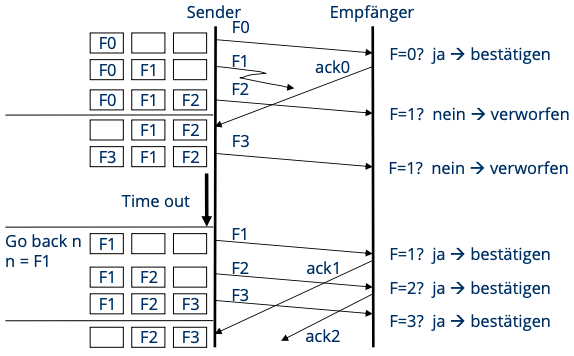
\includegraphics[width=0.75\textwidth]{./pics/TCP-Schiebefenster}
		\end{center}
		\item Sollten alle Bestätigungen zu $F$ gesendeten Paketen verloren gehen, fängt der Sender nach einem Timeout an, diese Daten nochmal zu senden und beginnt bei Laufnummer 0. Der Empfänger weiß aber nicht, ob das Paket mit der Nummer 0, was er gerade erhält, davon kommt, dass die Bestätigung zu den letzten $F$ Paketen nicht ankam und deswegen die Strategie \textit{go-back-n} sagt, dass die letzten $F$ Pakete nochmal geschickt werden müssen, oder ob die Laufnummer einfach nur das nächste Paket ist, was der Sender sendet und alle Bestätigungen angekommen sind.
		\item 100 \% Auslastung bedeutet, dass der 4. Frame gesendet wird, wenn ACK$_0$ ankommt. Das heißt, nachdem F0 abgesendet wurde, muss das Paket zum Empfänger laufen und die Bestätigung zum Sender zurück, insgesamt 40 ms. Währenddessen können F1, F2 und F3 bereits auf den Weg gebracht werden. Während also F0 in der Leitung ist, können 40 ms $\cdot$ 40 kBit/s = 1600 Bit geschickt werden. Diese 1600 Bit entsprechen aber 3 Frames, also ist ein Frame $F=\frac{4000}{3}\text{ Bit} = 534 \text{ Bit}$ groß.
		\begin{center}
			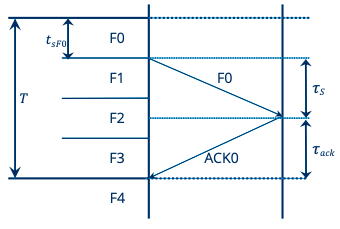
\includegraphics[width=0.6\textwidth]{./pics/Schiebefenster}
		\end{center}
	\end{enumerate}

	\section*{Aufgabe 4}
	\begin{enumerate}[label=(\alph*)]
		\item Ablauf
		\begin{center}
			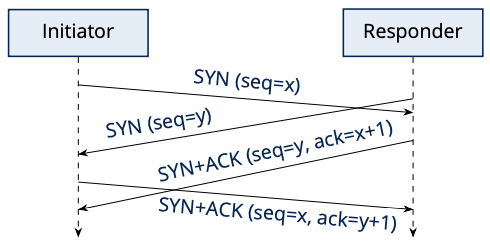
\includegraphics[width=0.75\textwidth]{./pics/gleichzeitig-TCP}
		\end{center}
		\item P1=64000 $\to$ gewünschte Puffergröße 64000 Byte, seq: gesendete Bytes eines Datenstroms, ack: nächste erwartete Bytes, das SYN-Segment gilt als 1 Byte des Datenstroms, deshalb stehen die Zähler nach dem Verbindungsaufbau auf x+1 und y+1
		\begin{center}
			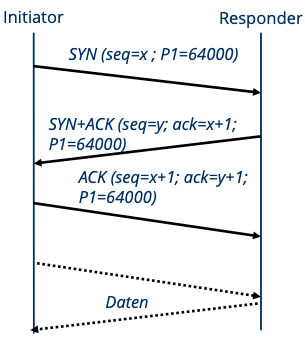
\includegraphics[width=0.65\textwidth]{./pics/TCPP-Verbindungsaufbau}
		\end{center}
		Datenübertragung
		\begin{center}
			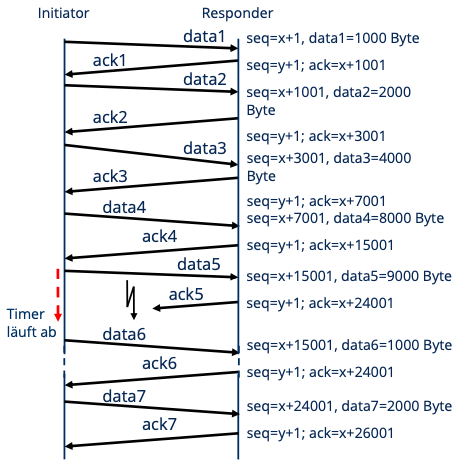
\includegraphics[width=0.75\textwidth]{./pics/TCPP-Datentransfer}
		\end{center}
		Verbindungsabbau
		\begin{center}
			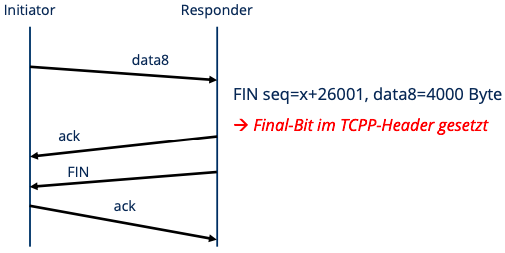
\includegraphics[width=0.75\textwidth]{./pics/TCPP-Verbindungsabbau}
		\end{center}
	\end{enumerate}

	\section*{Aufgabe 5}
	\begin{enumerate}[label=(\alph*)]
		\item P$_1$, P$_2$, …, P$_N$ sind Parameter, hier P$_1$ = 1200 Byte/s, P$_2$ = verschlüsselt
		\begin{center}
			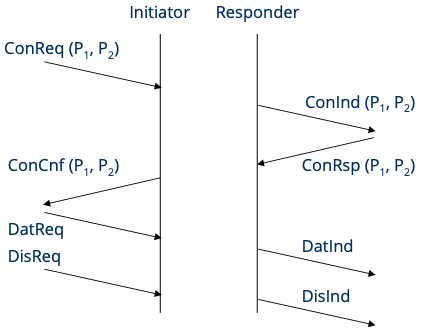
\includegraphics[width=0.65\textwidth]{./pics/QoS-1}
		\end{center}
		\item Responder ändert Datenrate auf 75 \% $\to$ Initiator akzeptiert $\to$ Verbindung existiert zu reduzierter Datenrate \\
		Responder ändert Datenrate auf 75 \% $\to$ Initiator akzeptiert nicht $\to$ Initiator baut Verbindung ab \\
		Responder kann geforderte Dienstgüte (Verschlüsselung) nicht erbringen $\to$ Abbruch der Verbindung
		\begin{center}
			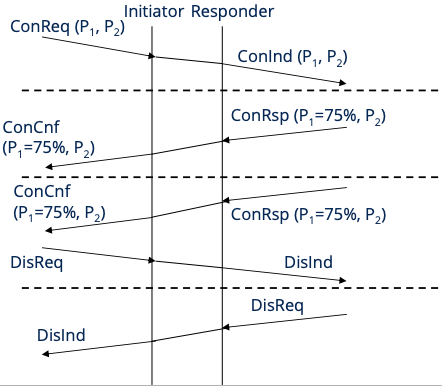
\includegraphics[width=0.65\textwidth]{./pics/QoS-2}
		\end{center}
	\end{enumerate}
	
\end{document}